% !TEX root = top.tex
% above command is so that compilation is always from top.tex
\section{Background} \label{sec:design}

In this section we describe the platforms HyperFork is built upon, including an
overview of the KVM hypervisor and kvmtool virtual machine monitor.

\subsection{KVM Overview}

% TODO KVM is ......

A full KVM system contains a number of major components within a Linux host
machine, as depicted in Figure~\ref{fig:kvm-arch}. The KVM kernel module tracks
and maintains most of the sensitive virtualized machine state. Each guest is
isolated within a standard linux process, which contains both VMM management components
as well as the running guest. Within the VMM, management components within the
userspace guest processes communicate with the KVM kernel module via a set of
ioctls. Outside of the guest processes, the VMM contains CLI based management
utility programs for administrators which use IPCs to communicate with the
guest process VMM components. For our implementation, the userspace VMM
components are implemented in kvmtool, however these same fundamental
components will exist in other KVM VMM implementations such as
Firecracker~\cite{firecracker}.

\begin{figure*}[t]
  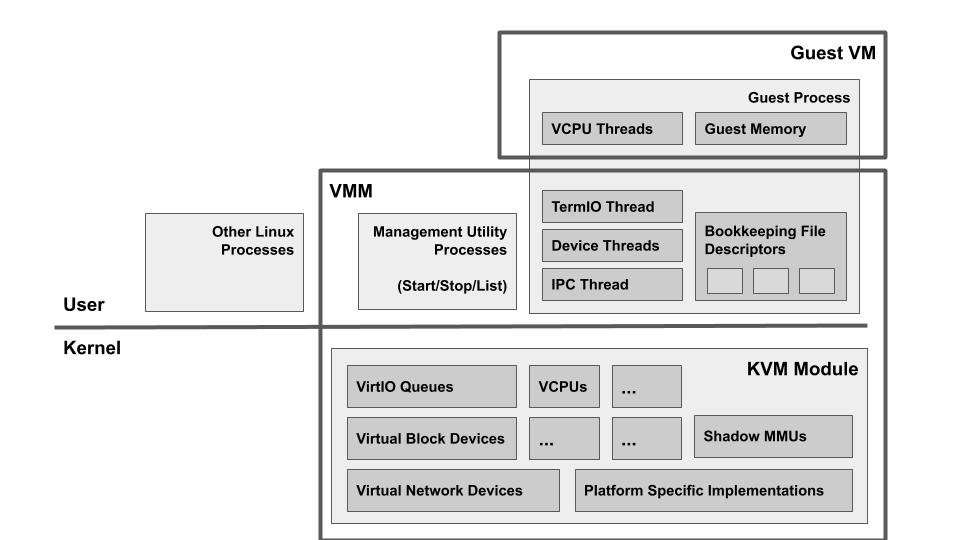
\includegraphics[width=0.8\textwidth]{{figures/kvm-arch}}
  \caption{KVM Software Architecture}
  \label{fig:kvm-arch}
\end{figure*}

\subsection{kvmtool}

kvmtool~\cite{kvmtool} is a VMM implementation for KVM with the minimal
functionality required to boot a fully functional linux kernel with very basic
virtualized devices. Supported devices include block, network, filesystem,
balloon, hardware random number generation, and console virtual devices, along
with a legacy 8250 serial device. kvmtool is provided as an alternative to
heavier VMM solutions such as QEMU~\cite{qemu}, which supports a wide range of
legacy devices and guest configurations.

We selected kvmtool as our userspace VMM as it offers a very similar set of
functionality to Firecracker, the VMM used to power Amazon Lambda. (TODO:
contrast firecracker and kvmtool) We chose kvmtool over Firecracker because we
found that Firecracker was more difficult to work with due to its Rust codebase
and containerization schemes. kvmtool provides a minimal platform on which to
test HyperFork applied to Linux guests and closely approximates the VMM of an
industrial serverless platform.

To virtualize efficiently, kvmtool makes use of a number of threads for
managing vCPUs and emulated devices. Userspace bookkeeping data structures hold
file descriptors which point to the internal VM state maintained within the KVM
kernel module. When the virtual machine is started, kvmtool creates a thread
for each class of device, including the terminal, 8250 serial console, block
devices, and other virtio devices. It then creates several worker threads to
handle arbitrary jobs that may arise from the virtio devices. These tasks
include processing work items from virtio queues and updating the console. In
its default configuration, kvmtool allocates one worker thread for each CPU on
the host machine. As we are virtualizing machines that are much smaller than
the host machine, we limited kvmtool to one worker thread per VM. In addition
to device threads, kvmtool also creates a thread to manage the virtual machines
through IPC calls. This allows administrators to start, pause, stop, and debug
virtual machines using a simple command line interface. Finally, kvmtool
creates one thread per vCPU that proceeds in a loop, invoking the
\texttt{KVM\_RUN} ioctl, then handling any IO requests or interrupts that may
arise. Together, this set of threads enables efficient virtualization of the
guest and its devices.

